\Oznaka{}{Hip}{}
\Rokovi{2017-I2, 2017-I3, 2017-I5, 2018-I2, 2020-S6}
\Tekst{
Kolica mase $150\ kg$ postavljena na tračnice pomaknu se za $20\ m$ pod djelovanjem stalne sile iznosa $\vec{F}_0=200 \ N$ koja djeluje pod kutom $30^\circ$ od  prema tračnicama (vidjeti skicu – pogled odozgora). Koliki je iznos konačne brzine kolica ako su krenula iz stanja mirovanja? (Trenje po tračnicama i otpor zraka se zanemaruju.)

\begin{figure}[h]%{r}{0.4\textwidth} % Inline image example
  \begin{center}
    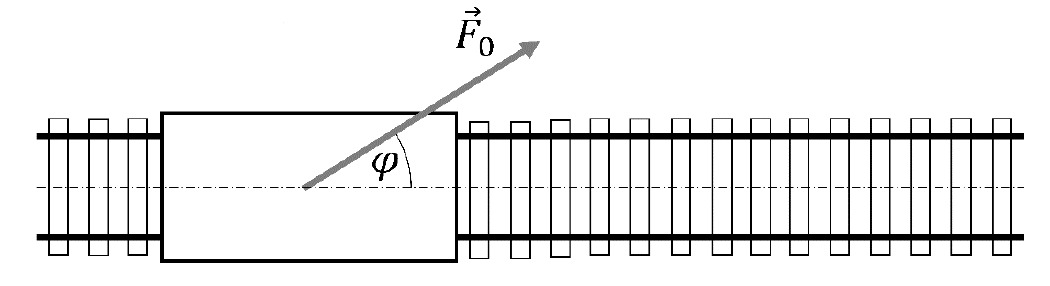
\includegraphics[scale=0.29]{../04_Zakoni_ocuvanja/Zadatak_C210.png}
  \end{center}
\end{figure}

}
\Rjesenje{$\vec{v}=6,796\ ms^{-1} $}
\Postupak{

}

